\section{Decision Trees and Gradient Boosting}
\subsection{Decision Trees}
\ac{DT} are, similarly to \ac{NN} one of the most popular \ac{ML} methods used today.
Contrary to \ac{NN}, \ac{DT} are famously easy in theory. Despite the simplicity of \ac{DT}, 
they are capable of solving a large range of complex problems. In this section I will cover the use 
of \ac{DT} as applied to a supervised classification problem.
\\
The goal of decision trees are to create a flowchart-like tree structure from input to output. 
Similarly to the traditional cut-and-count method used in particle physics, a \ac{DT} 
places \emph{rectangular-cuts} on a data set. It does so to create a collection of thresholds 
$\bf{\mathcal{C}} \sf =\{c_1, c_2,...,c_{N_c}\}$, which when applied to a new data set and target, 
will sort each data point to the corresponding target. 
\\
In figure \ref{fig:DT}, I have illustrated a simple \ac{DT} classifying a 4-dimensional 
input data to one of three classifications. As is visualized in figure \ref{fig:DT}, the \ac{DT} 
applies a set of thresholds on the data to find the route applicable to a target. For each applied 
cut, the data split into what we call \emph{branches}. Each branch represents a subset of the data.
The final subset, after a sufficient amount of cuts ends in what we call \emph{leaves}. The leaves are 
the label we assign the subset of data contained in this branch.
\\  
\begin{figure}
    \centering
    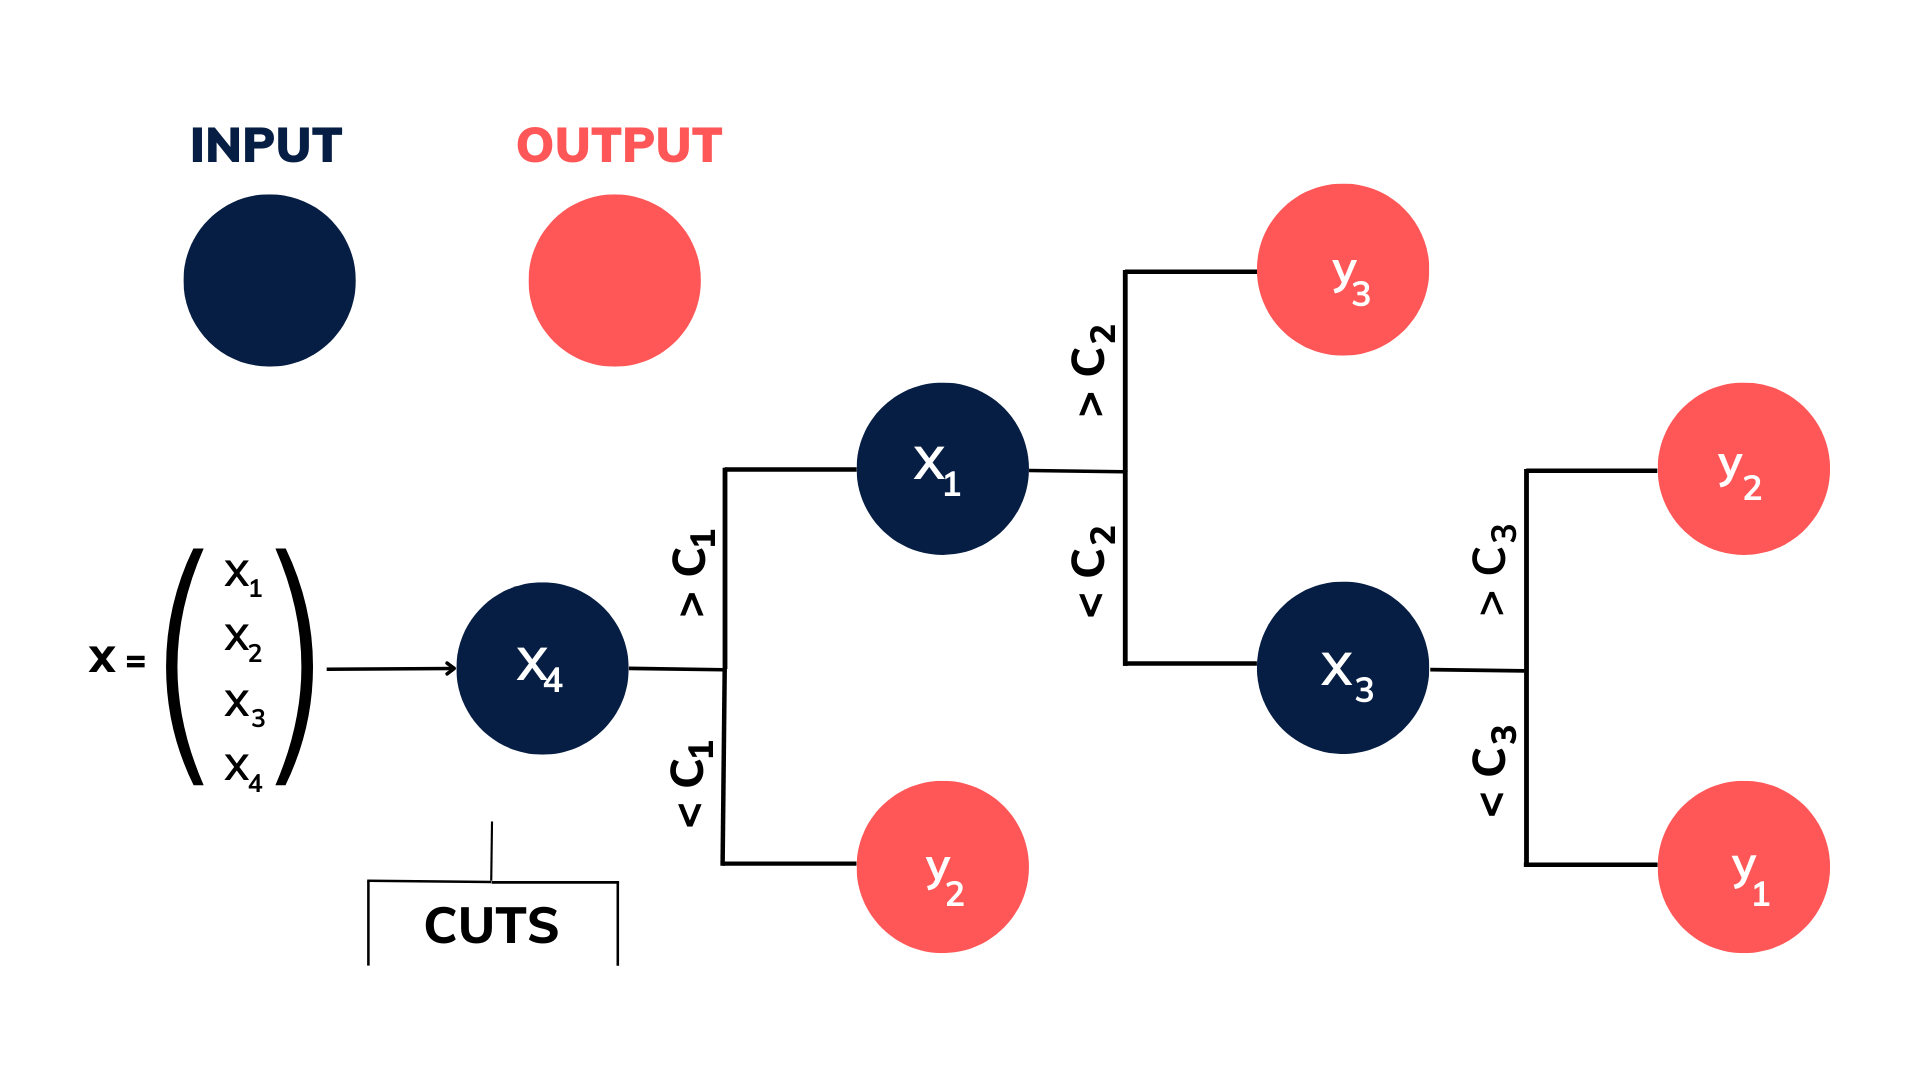
\includegraphics[width=0.6\textwidth]{Figures/Illustrations/DT.png}
    \caption{An illustration of a simple \ac{DT}, mapping a 4 dimensional input 
    to one of three values in the target space.}
    \label{fig:DT}
\end{figure}
Just like most \ac{ML}-methods, there are many kinds of \ac{DT} each with their own 
architecture and benefits. In the case of \ac{DT} the defining qualities can be summarized in
its choice of \emph{Deepness} and \emph{Optimization}. When provided with a data set,
a \ac{DT} can in theory create as many cuts needed to map each individual data point, $\textbf{x}_i$ to the 
corresponding target, $t_i$. Doing so would not only be very computationally heavy, but would almost 
certainly lead to overfitting if applied to any new data. Instead, when building a \ac{DT} one defines 
a maximum deepness. This means that we must define a limit to the length of $\bf \mathcal{C}$, which 
subsequently leads to the need for a prioritization of cuts. 
\\
Building a \ac{DT} and choosing which cuts to apply at what point, is the equivalent of training a 
network. How to decide by what standard one chooses to building the hierarchy of cuts is again the 
equivalent of choosing an optimizer. For more information on \ac{DT}'s, the reader is referred to the 
book by Hastie et al. \cite{huang_introduction_2014}.
\subsection{Gradient Boosting in Decision Trees}
Gradient-boosting is an algorithm which uses a collective of "weak" 
classifiers in order to create one strong classifier. In the case of gradient-boosted 
trees the weak classifiers are a collective of shallow trees, which combine to form a classifier 
that allows for deeper learning. As is the case for most gradient-boosting 
techniques, the collecting of weak classifiers is an iterative process.
\\
We define an imperfect model $\mathcal{F}_m$, which is a collection of m number of weak 
classifiers, estimators. A prediction for the model on a given data-points, $\textbf{x}_i$ is 
defined as $\mathcal{F}_m(\textbf{x}_i)$, and the target for the aforementioned data is 
defined as $t_i$. The goal of the iterative process is to minimize some cost-function 
$\mathcal{C}$ by introducing a new estimator $h_m$ to compensate for any error, 
$\mathcal{C}(\mathcal{F}_m(\textbf{x}_i), y_i)$. In other words we define the new estimator as:
\begin{align}
    \tilde{\mathcal{C}}(\mathcal{F}_m(\textbf{x}_i), \textbf{y}_i) = h_m(\textbf{x}_i),
\end{align}
where we define $\tilde{\mathcal{C}}$ as some relation defined between the observed and 
predicted values such that when added to the initial prediction we minimize $\mathcal{C}$.
\\
Using our new estimator $h_m$, we can now define a new model as
\begin{align}
    \mathcal{F}_{m+1}(\textbf{x}_i) = \mathcal{F}_m + h_m (\textbf{x}_i).
\end{align}
Similarly to how we define a deepness of trees, we can define the degree of boosting. We define 
this as the amount of trees used in the iterative process, or M. This means that the final classifier 
becomes
\begin{align}
    \mathcal{F}_M (\textbf{x}_i) = \sum_{i=0}^M h_i(\textbf{x}_i)
\end{align} 
The XGBoost \cite{XGB} framework used in this analysis enables a (advanced) gradient-boosted algorithm, 
and was initially created for the Higgs ML challenge. Since the challenge, XGBoost has become 
a favorite for many in the ML community and has later won many other ML challenges. XGBoost 
often outperforms ordinary decision trees, but what is gains in results it looses in 
interpretability. A single tree can easily be analyzed and dissected, but when the number 
of trees increases this becomes harder. For more detailed explanation on the XGBoost framework,
the reader is referred to Ref.\cite{XGB}